\chapter{भोजन की यात्रा}\label{ch:g4:journey-of-food}

रोटी का एक कौर: चबाया, निगला --- और ग़ायब। ग़ायब कहाँ? आज रात तक उस
रोटी का कुछ हिस्सा तुम्हारी \omterm{def:g1:my-body:parts}{टाँगों} को दौड़ाने और तुम्हारी \omterm{def:g3:bones-and-muscles:skeleton}{हड्डियों} को
बढ़ाने में लगा होगा, यानी उसे किसी तरह उस नली से \emph{बाहर} निकलकर
बाक़ी शरीर के \emph{भीतर} पहुँचना ही पड़ेगा जिसमें उसे निगला गया था।
कौर के पीछे-पीछे चलो: उसकी यात्रा शरीर की सबसे अच्छी कहानियों में से
एक है।

\section{पाचन नली}

\begin{definition}[पाचन नली]\label{def:g4:journey-of-food:tract}
भोजन \emph{पाचन नली}\index{पाचन नली} से होकर सफ़र करता है, जो पूरे शरीर
से होकर गुज़रती एक लंबी नली है:
\begin{enumerate}
  \item \emph{मुँह}\index{मुँह}, जहाँ दाँत पीसते हैं
        (\cref{ch:g2:teeth-and-eating-well}) और \emph{लार}\index{लार}
        गीला करती है;
  \item \emph{ग्रासनली}\index{ग्रासनली}, गले से आमाशय तक की फिसलपट्टी;
  \item \emph{आमाशय}\index{आमाशय}, एक पेशीदार थैली, जहाँ भोजन घंटों
        मथा जाता है और पाचक रसों में मिलाया जाता है;
  \item \emph{छोटी आँत}\index{छोटी आँत}, कई मीटर लंबी तह की हुई नली,
        जहाँ \omterm{def:g4:journey-of-food:digestion}{पाचन} पूरा होता है और भोजन का सार शरीर में उतर जाता है;
  \item \emph{बड़ी आँत}\index{बड़ी आँत}, जहाँ बचे हुए से पानी वापस ले
        लिया जाता है, और फिर बचा-खुचा शरीर से बाहर चला जाता है।
\end{enumerate}
\end{definition}

\begin{omfigure}
\begin{tikzpicture}
  \node[anchor=south west, inner sep=0] (img) at (0,0)
    {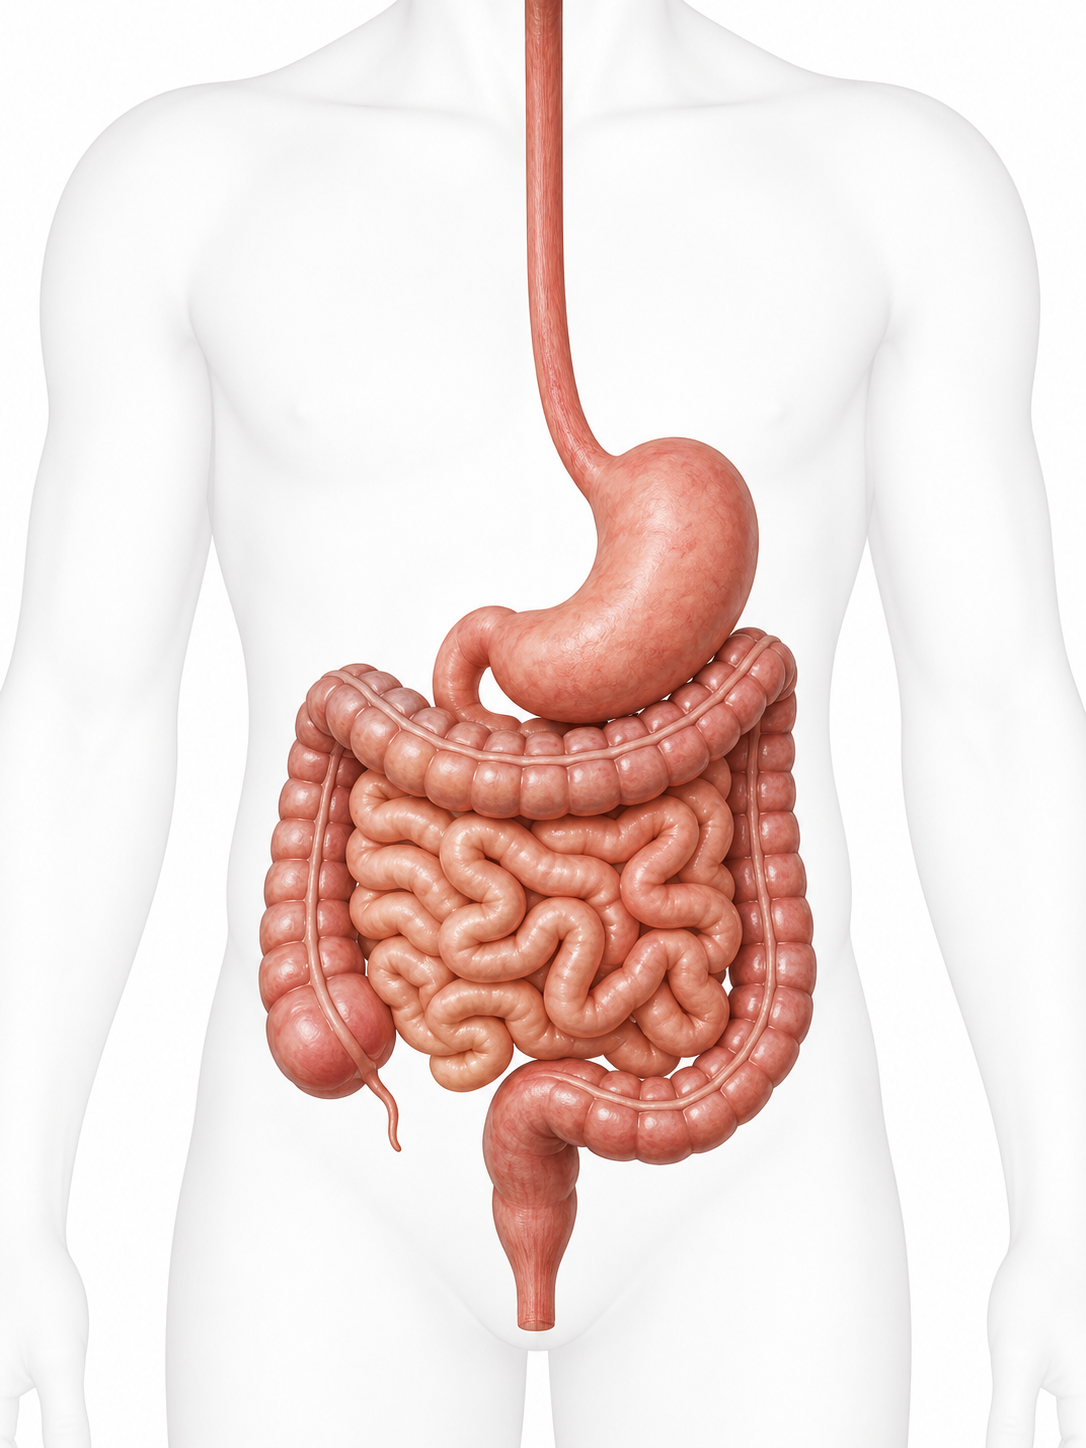
\includegraphics[width=0.5\linewidth]{images/book1/ai/fig-digestive.png}};
  \begin{scope}[x={(img.south east)}, y={(img.north west)},
      every node/.style={font=\small}]
    \draw[omDef, thick] (0.52,0.85) -- (0.72,0.88) node[right] {ग्रासनली};
    \draw[omDef, thick] (0.66,0.62) -- (0.82,0.66) node[right] {आमाशय};
    \draw[omDef, thick] (0.44,0.35) -- (0.16,0.28)
      node[left, align=center] {छोटी आँत\\ (कई मीटर, तह की हुई)};
    \draw[omDef, thick] (0.74,0.42) -- (1.04,0.40)
      node[right, align=left] {बड़ी\\ आँत};
    \draw[omDef, thick] (0.50,0.09) -- (0.66,0.05)
      node[right] {बचा-खुचा बाहर};
  \end{scope}
\end{tikzpicture}

{\small \omterm{def:g4:journey-of-food:tract}{पाचन नली}: मुँह से निकास तक एक ही नली। \omterm{def:g4:journey-of-food:tract}{ग्रासनली} \omterm{def:g4:journey-of-food:tract}{आमाशय} तक
पहुँचाती है; \omterm{def:g4:journey-of-food:tract}{छोटी आँत} के तह किए मीटर बीच का हिस्सा भरते हैं, और उनके
चारों ओर \omterm{def:g4:journey-of-food:tract}{बड़ी आँत} का चौखटा है।}
\end{omfigure}

\begin{example}[यात्रा का समय]\label{ex:g4:journey-of-food:timing}
रोटी का कौर मुँह में सेकंड भर रहता है, \omterm{def:g4:journey-of-food:tract}{ग्रासनली} से फिसलने में कुछ
सेकंड लेता है, \omterm{def:g4:journey-of-food:tract}{आमाशय} में कुछ घंटे मथा जाता है, \omterm{def:g4:journey-of-food:tract}{छोटी आँत} से गुज़रने में
कई घंटे और लगाता है, और \omterm{def:g4:journey-of-food:tract}{बड़ी आँत} में एक दिन या उससे भी ज़्यादा लेकर
पूरा होता है। पूरी यात्रा में आम तौर पर एक से दो दिन लगते हैं।
\end{example}

\section{पाचन: भोजन से पोषक तत्वों तक}

\begin{definition}[पाचन और पोषक तत्व]\label{def:g4:journey-of-food:digestion}
\emph{पाचन}\index{पाचन} भोजन का, नली के साथ-साथ, इतने छोटे और सरल
घटकों में बदल जाना है कि वे शरीर में उतर सकें: यही
\emph{पोषक तत्व}\index{पोषक तत्व} हैं। दाँत और \omterm{def:g4:journey-of-food:tract}{आमाशय} का मथना भोजन को
तोड़ते हैं; \emph{पाचक रस}\index{पाचक रस} --- जिनमें \omterm{def:g4:journey-of-food:tract}{लार} भी है ---
उसे टुकड़ा-टुकड़ा करके और आगे खोलते जाते हैं, जब तक जो रोटी थी वह पोषक
तत्वों का तरल मेल न बन जाए।
\end{definition}

\begin{example}[रोटी मीठी हो जाती है]\label{ex:g4:journey-of-food:sweet}
सादी रोटी का एक टुकड़ा बहुत देर तक चबाओ --- धीरे-धीरे साठ तक गिनने भर
--- और हलकी-सी मिठास आ जाती है। कुछ मिलाया नहीं गया: \omterm{def:g4:journey-of-food:tract}{लार} पहले ही रोटी
को सरल, मीठे टुकड़ों में खोल रही है। तुमने \omterm{def:g4:journey-of-food:digestion}{पाचन} को शुरू होते हुए चख
लिया।
\end{example}

\begin{proposition}[शरीर में उतरना]\label{prop:g4:journey-of-food:absorb}
नली का भीतरी हिस्सा एक तरह से अब भी शरीर के बाहर ही है --- डोनट के
छेद की तरह। उतरना \emph{\omterm{def:g4:journey-of-food:tract}{छोटी आँत}} में होता है: उसकी पतली, गहरी तह वाली
दीवारों से \omterm{def:g4:journey-of-food:digestion}{पोषक तत्व} \emph{रक्त}\index{रक्त} में उतर जाते हैं, और \omterm{prop:g4:journey-of-food:absorb}{रक्त}
उन्हें शरीर के हर हिस्से तक पहुँचाता है (यही वह पहुँचाने की सेवा है
जिसे \cref{ch:g4:heart-and-blood} खोलता है)। जो नहीं उतर सकता ---
रेशे, भूसी --- वह आगे बढ़ता है, \omterm{def:g4:journey-of-food:tract}{बड़ी आँत} में अपना पानी गँवाता है, और
मल के रूप में बाहर निकल जाता है।
\end{proposition}
\admitted

\begin{remark}[तहें और मीटर क्यों]\label{rem:g4:journey-of-food:surface}
उतरने के लिए दीवार का क्षेत्रफल चाहिए, और \omterm{def:g4:journey-of-food:tract}{छोटी आँत} इसी के लिए बनी है:
कई मीटर की लंबाई, और भीतर से तह पर तह पड़ी दीवारें। सपाट फैला दो तो
यह उतरने वाली सतह एक छोटे कमरे में क़ालीन की तरह बिछ जाए --- और वह
तुम्हारे पेट में भरी हुई है। शरीर में बड़े काम बड़ी सतहों को छोटा
समेटकर होते हैं।
\end{remark}

\section{पाचन का काम आसान करना}

\begin{method}[पाचन के अनुकूल आदतें]\label{met:g4:journey-of-food:habits}
\begin{enumerate}
  \item ठीक से चबाओ: \omterm{def:g4:journey-of-food:tract}{आमाशय} के दाँत नहीं होते --- मुँह जो छोड़ देता है,
        उससे \omterm{def:g4:journey-of-food:tract}{आमाशय} को जूझना पड़ता है;
  \item शांति से, तय समय पर खाओ;
  \item खाने के साथ पानी पियो;
  \item रेशेदार भोजन खाओ --- सब्ज़ियाँ, \omterm{prop:g3:flowers-fruits-seeds:transform}{फल}, चोकर वाली रोटी: रेशा
        बचे-खुचे को चलता रखता है;
  \item कड़ा खेल या तैराकी खाना बैठ जाने के बाद के लिए छोड़ो: मेहनत
        करता \omterm{def:g4:journey-of-food:tract}{आमाशय} और मेहनत करती \omterm{def:g1:my-body:parts}{टाँगें} आपस में होड़ करते हैं।
\end{enumerate}
\end{method}

\begin{example}[पेटदर्द का जासूस]\label{ex:g4:journey-of-food:ache}
जल्दी-जल्दी निगला हुआ दोपहर का खाना, और फिर दौड़: दोपहर बाद का वही
जाना-पहचाना पेटदर्द। खाना आधा चबाकर निगला गया (नियम 1 टूटा) और पचाते
हुए \omterm{def:g4:journey-of-food:tract}{आमाशय} को दौड़ में झोंक दिया गया (नियम 5)। इसका इलाज दवा नहीं,
अपनी ही \omterm{def:g4:journey-of-food:tract}{पाचन नली} के प्रति तमीज़ है।
\end{example}

\section{अभ्यास}

\begin{exercise}[$\star$]\label{exo:g4:journey-of-food:1}
\omterm{def:g4:journey-of-food:tract}{पाचन नली} के भागों के नाम मुँह से निकास तक क्रम से बताओ।
\end{exercise}

\begin{exercise}[$\star$]\label{exo:g4:journey-of-food:2}
\omterm{def:g4:journey-of-food:tract}{आमाशय} में भोजन का क्या होता है, और वह वहाँ लगभग कितनी देर रहता है?
\end{exercise}

\begin{exercise}[$\star$]\label{exo:g4:journey-of-food:3}
\omterm{def:g4:journey-of-food:digestion}{पाचन} क्या है? \omterm{def:g4:journey-of-food:digestion}{पोषक तत्व} क्या हैं?
\end{exercise}

\begin{exercise}[$\star$]\label{exo:g4:journey-of-food:4}
\omterm{def:g4:journey-of-food:digestion}{पोषक तत्व} किस भाग में \omterm{prop:g4:journey-of-food:absorb}{रक्त} में उतरते हैं? जो नहीं उतर सकता उसका क्या
होता है?
\end{exercise}

\begin{exercise}[$\star$]\label{exo:g4:journey-of-food:5}
देर तक चबाई गई रोटी हलकी मीठी क्यों हो जाती है?
\end{exercise}

\begin{exercise}[$\star$]\label{exo:g4:journey-of-food:6}
\omterm{def:g4:journey-of-food:tract}{छोटी आँत} इतनी लंबी और भीतर से इतनी तह वाली क्यों होती है?
\end{exercise}

\begin{exercise}[$\star$]\label{exo:g4:journey-of-food:7}
\omterm{def:g4:journey-of-food:digestion}{पाचन} के अनुकूल तीन आदतें और हर एक का कारण बताओ।
\end{exercise}

\begin{exercise}[$\star$]\label{exo:g4:journey-of-food:8}
करके देखो (खाने की मेज़ पर): अपने अगले खाने का समय नापो। तुम्हारा भोजन
तुम्हारे मुँह में कितनी देर रहता है --- और यह उसके आगे पड़े दिनों के
मुक़ाबले कैसा है?
\end{exercise}

\begin{exercise}[$\star\star$]\label{exo:g4:journey-of-food:9}
\cref{ex:g4:journey-of-food:ache} के पेटदर्द की जाँच करो: कौन-सी दो
आदतें टूटी थीं, और कल तुम क्या बदलोगे?
\end{exercise}

\begin{exercise}[$\star\star$]\label{exo:g4:journey-of-food:10}
``जैसे ही तुम निगलते हो, भोजन शरीर में चला जाता है।'' इसे
\cref{prop:g4:journey-of-food:absorb} से सुधारो: भोजन सचमुच शरीर में
कहाँ उतरता है, और उससे पहले उसके साथ क्या होना चाहिए?
\end{exercise}

\begin{exercise}[$\star\star\star$]\label{exo:g4:journey-of-food:11}
गाय की घास तुम्हारी रोटी से कहीं ज़्यादा सख़्त भोजन है --- और गाय के
\omterm{def:g4:journey-of-food:tract}{आमाशय} के चार कक्ष होते हैं, वह अपना भोजन दो बार चबाती है, और घास खोलने
के लिए अपनी आँत में मददगार \omterm{def:g1:living-or-not:living}{सजीव} बसाए रखती है।
\cref{def:g4:journey-of-food:digestion} और
\cref{prop:g2:what-animals-eat:match} से समझाओ कि घास खाने वाले को यह
भारी मशीनरी क्यों चाहिए।
\end{exercise}
